% !TEX root = thesis.tex

\chapter{Data analysis}
\label{cha:data_analysis}
The datasets created allow to perform some measurement regarding the use of scholarly works in the English Wikipedia.
\todo{TODO\@: other statistics? Maybe some that use the pagecounts?}

\section{Wikipedia articles}
\subsection{Where do identifiers appear in a Wikipedia article?}

\subsection{How many sections Wikipedia articles have?}

\subsection{Which are the most common sections in Wikipedia articles?}

\section{Papers in Wikipedia}
This section analyzes the use of papers in wikipedia.

\subsection{Incoming citations distribution}
Ciao
\begin{figure}[ht]
    \centering
    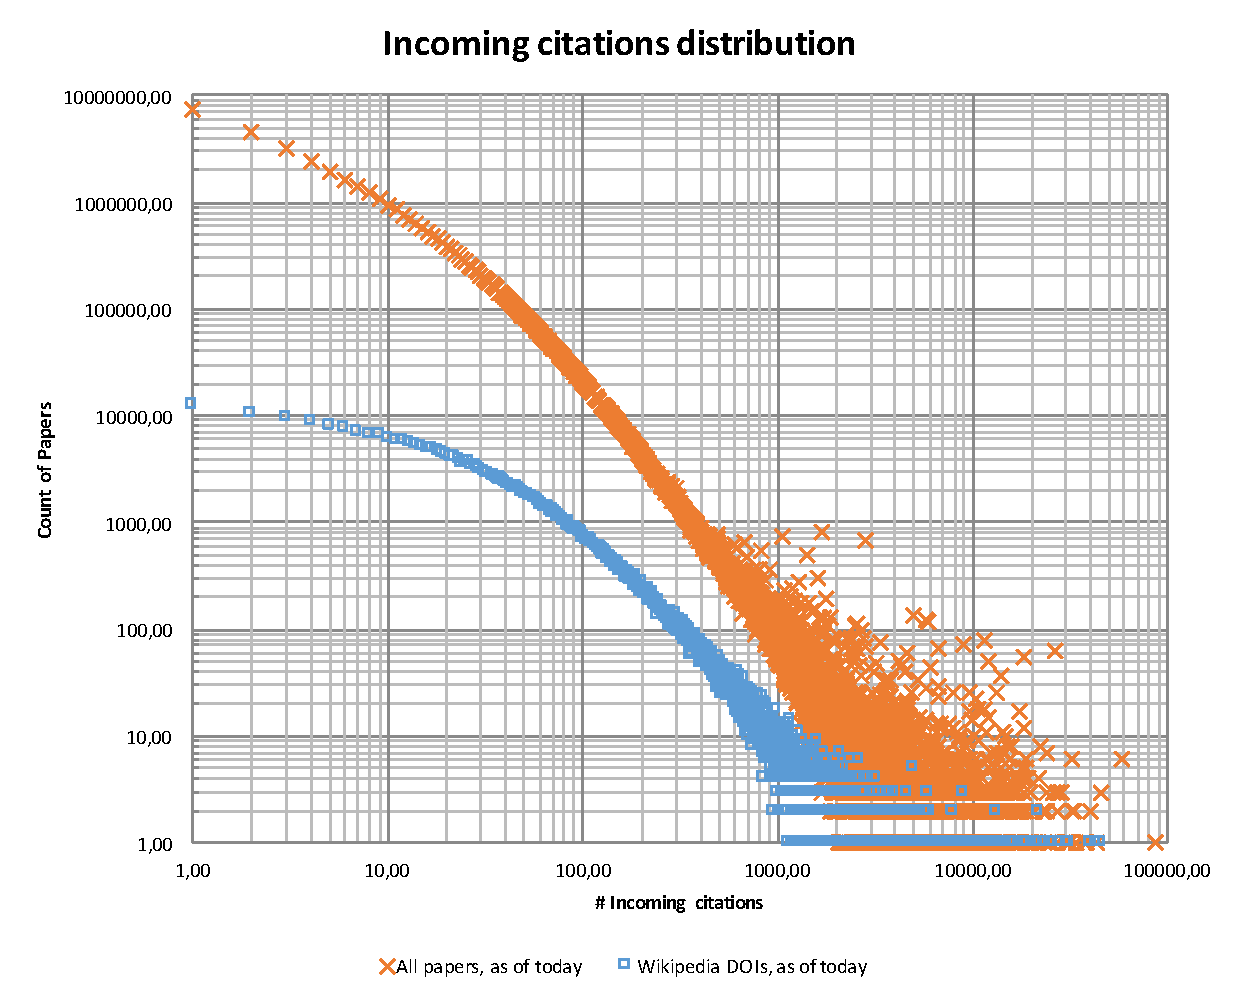
\includegraphics[keepaspectratio=true, width=\textwidth]{assets/incoming_cits}
    \caption{Incoming citations distribution of papers appearing in the \emph{mag} datasets and the ones appearing only in English Wikipedia, on a log-log scale.}
    \label{fig:incoming_citations_loglog}
\end{figure}

\begin{figure}[ht]
    \centering
    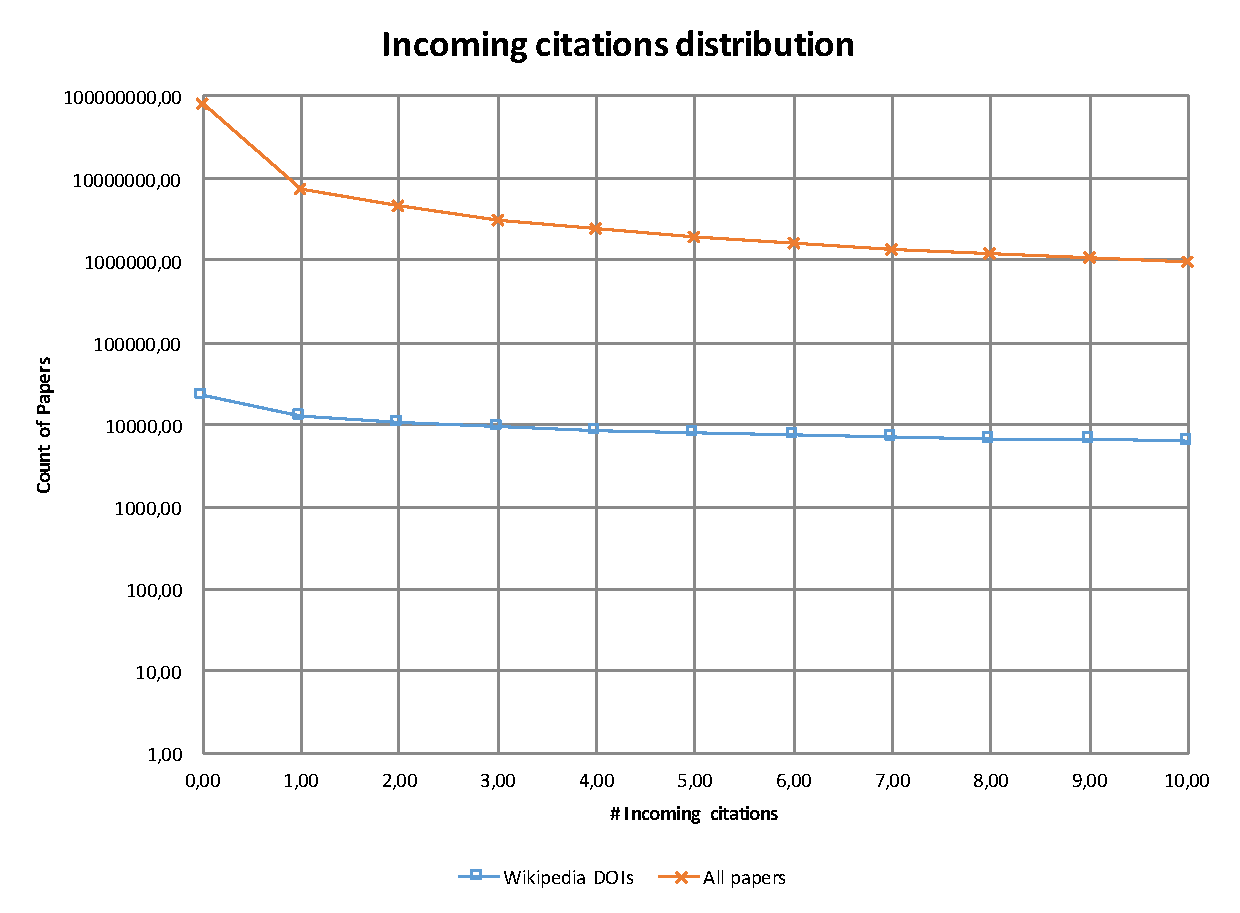
\includegraphics[keepaspectratio=true, width=\textwidth]{assets/incoming_cits_log}
    \caption{Incoming citations distribution of papers appearing in the \emph{mag} datasets and the ones appearing only in English Wikipedia, on a log scale on the Y axis.}
    \label{fig:incoming_citations_log}
\end{figure}

\subsection{Publication date distribution}

\subsection{Age at first appearance}

\subsection{Lifetime in a Wikipedia article}

\subsection{Top cited journals by views}
